\section{QoI Model}
\label{sec:qoi_model}

%\begin{figure}
%\centering
%    \subfigure[Sum Similarity]{
%        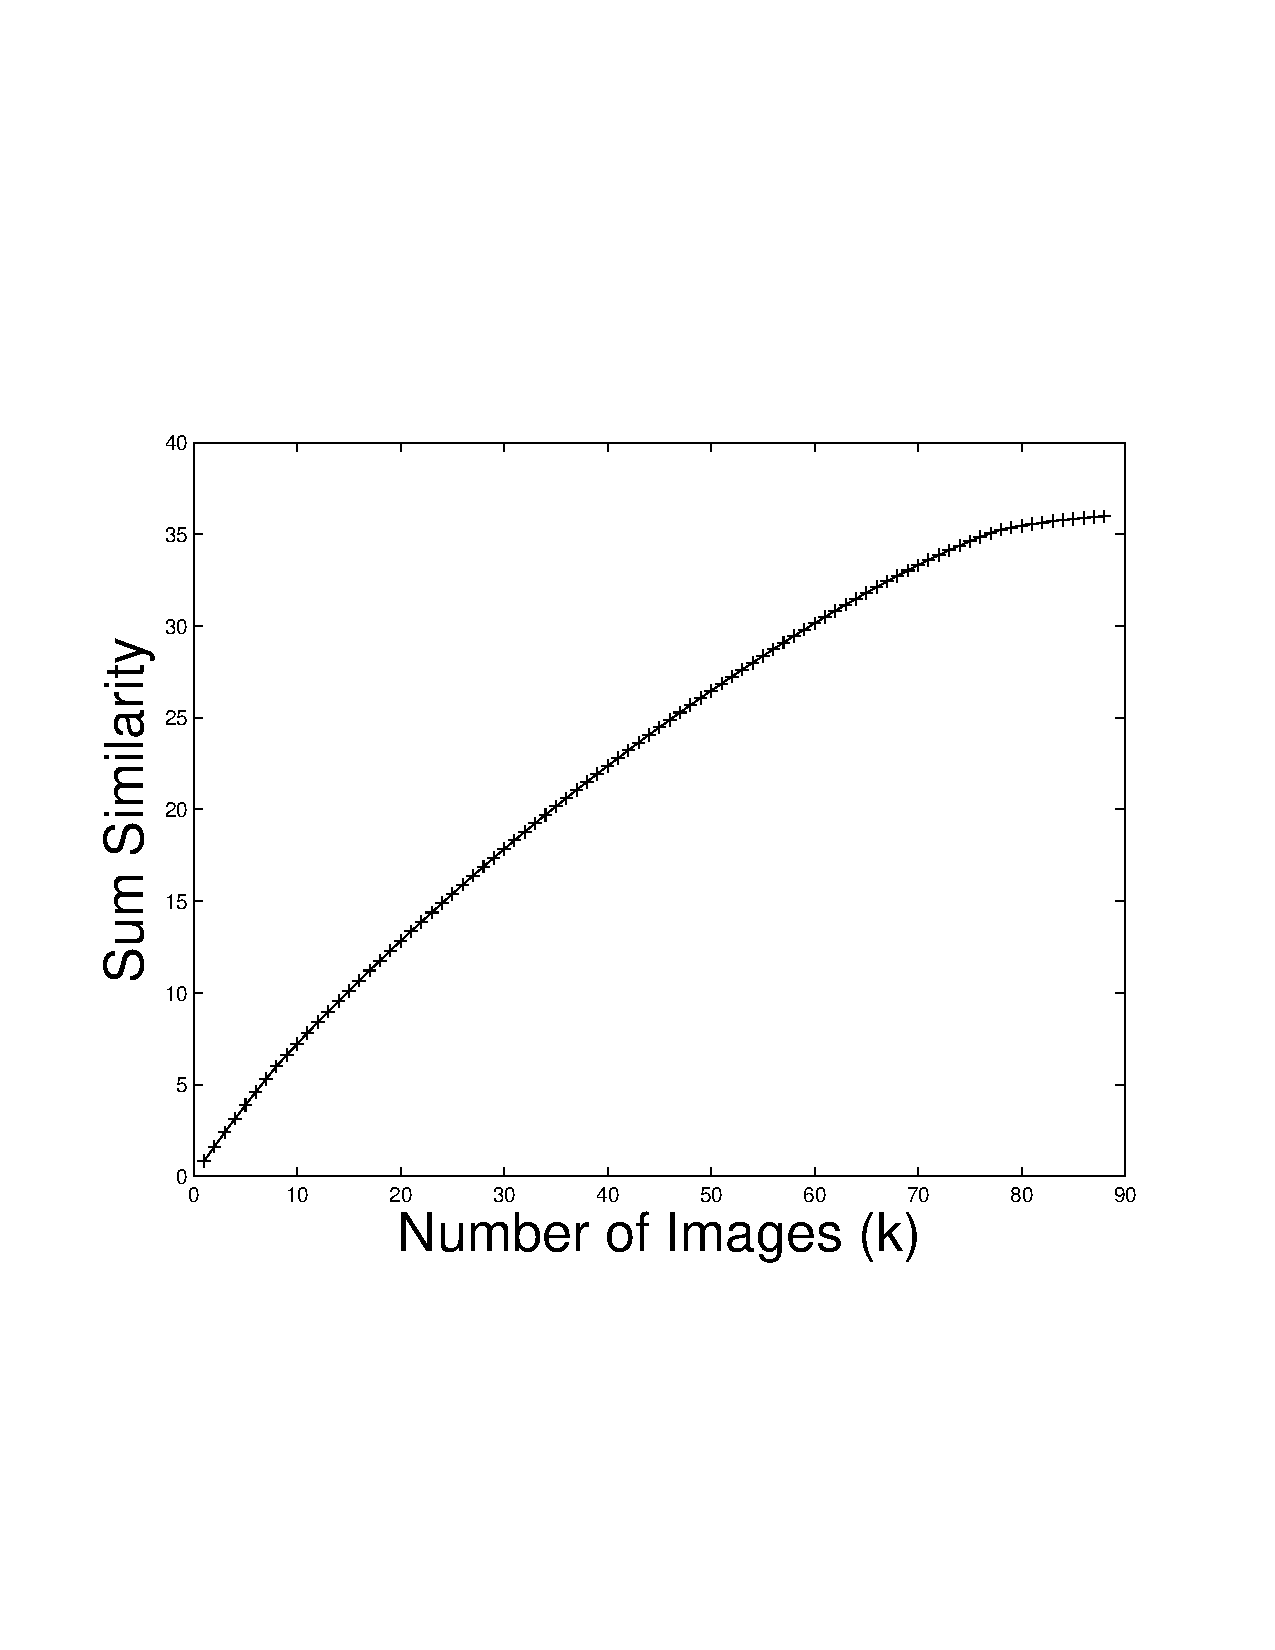
\includegraphics[clip=true, trim = 17mm 65mm 25mm 70mm, scale=0.23]{figures/topk/topk_sum_sim.pdf}
%        \label{fig:topkSumSim}
%        }
%    \subfigure[Avg. Match Target]{
%        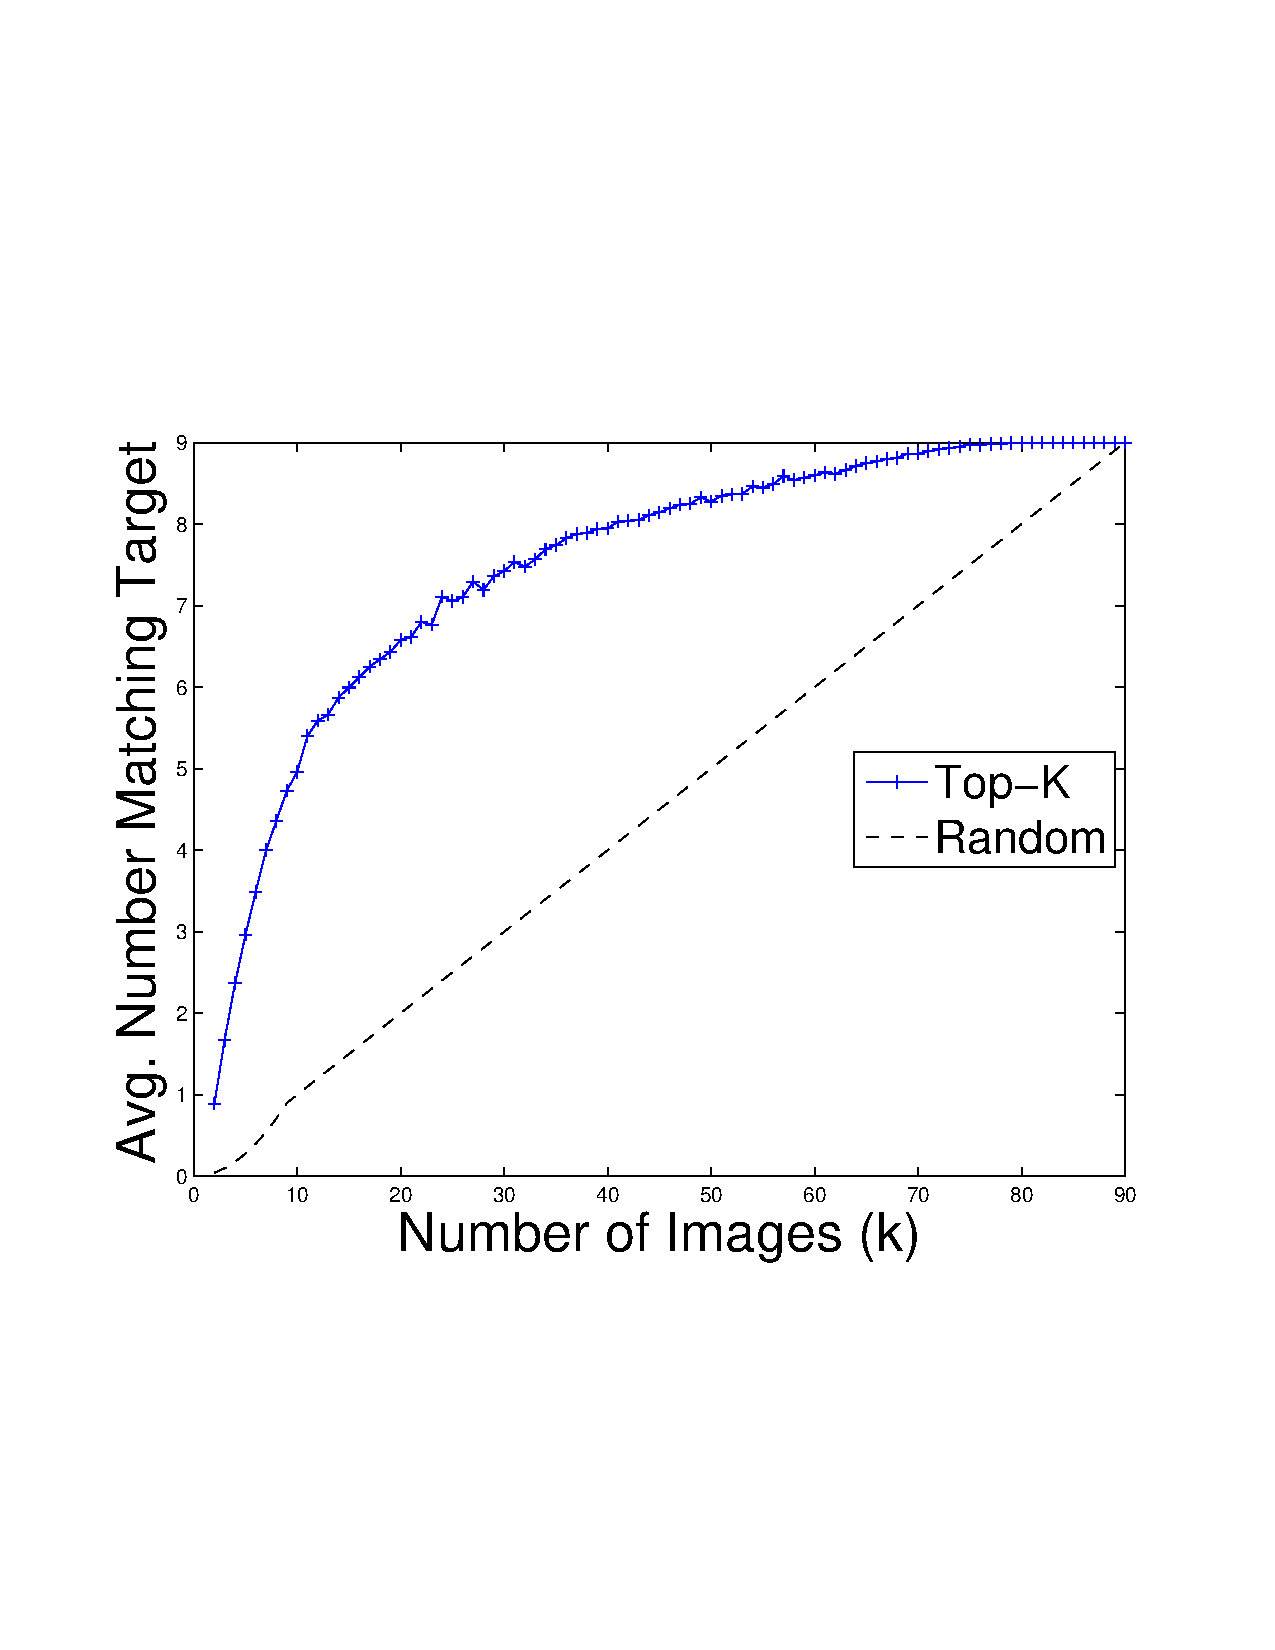
\includegraphics[clip=true, trim = 17mm 65mm 23mm 70mm, scale=0.23]{figures/topk/avg_num_matching_color.pdf}
%        \label{fig:topkAvgNumSameSet}
%        }
%   \caption{Completeness metrics for the Top-K selection algorithm. Each exhibits a diminishing return as more images are added.}
%   \label{fig:completeness_exp_results}
%\end{figure}

\begin{figure*}
\centering
    \subfigure[Top-K: Sum Similarity]{
        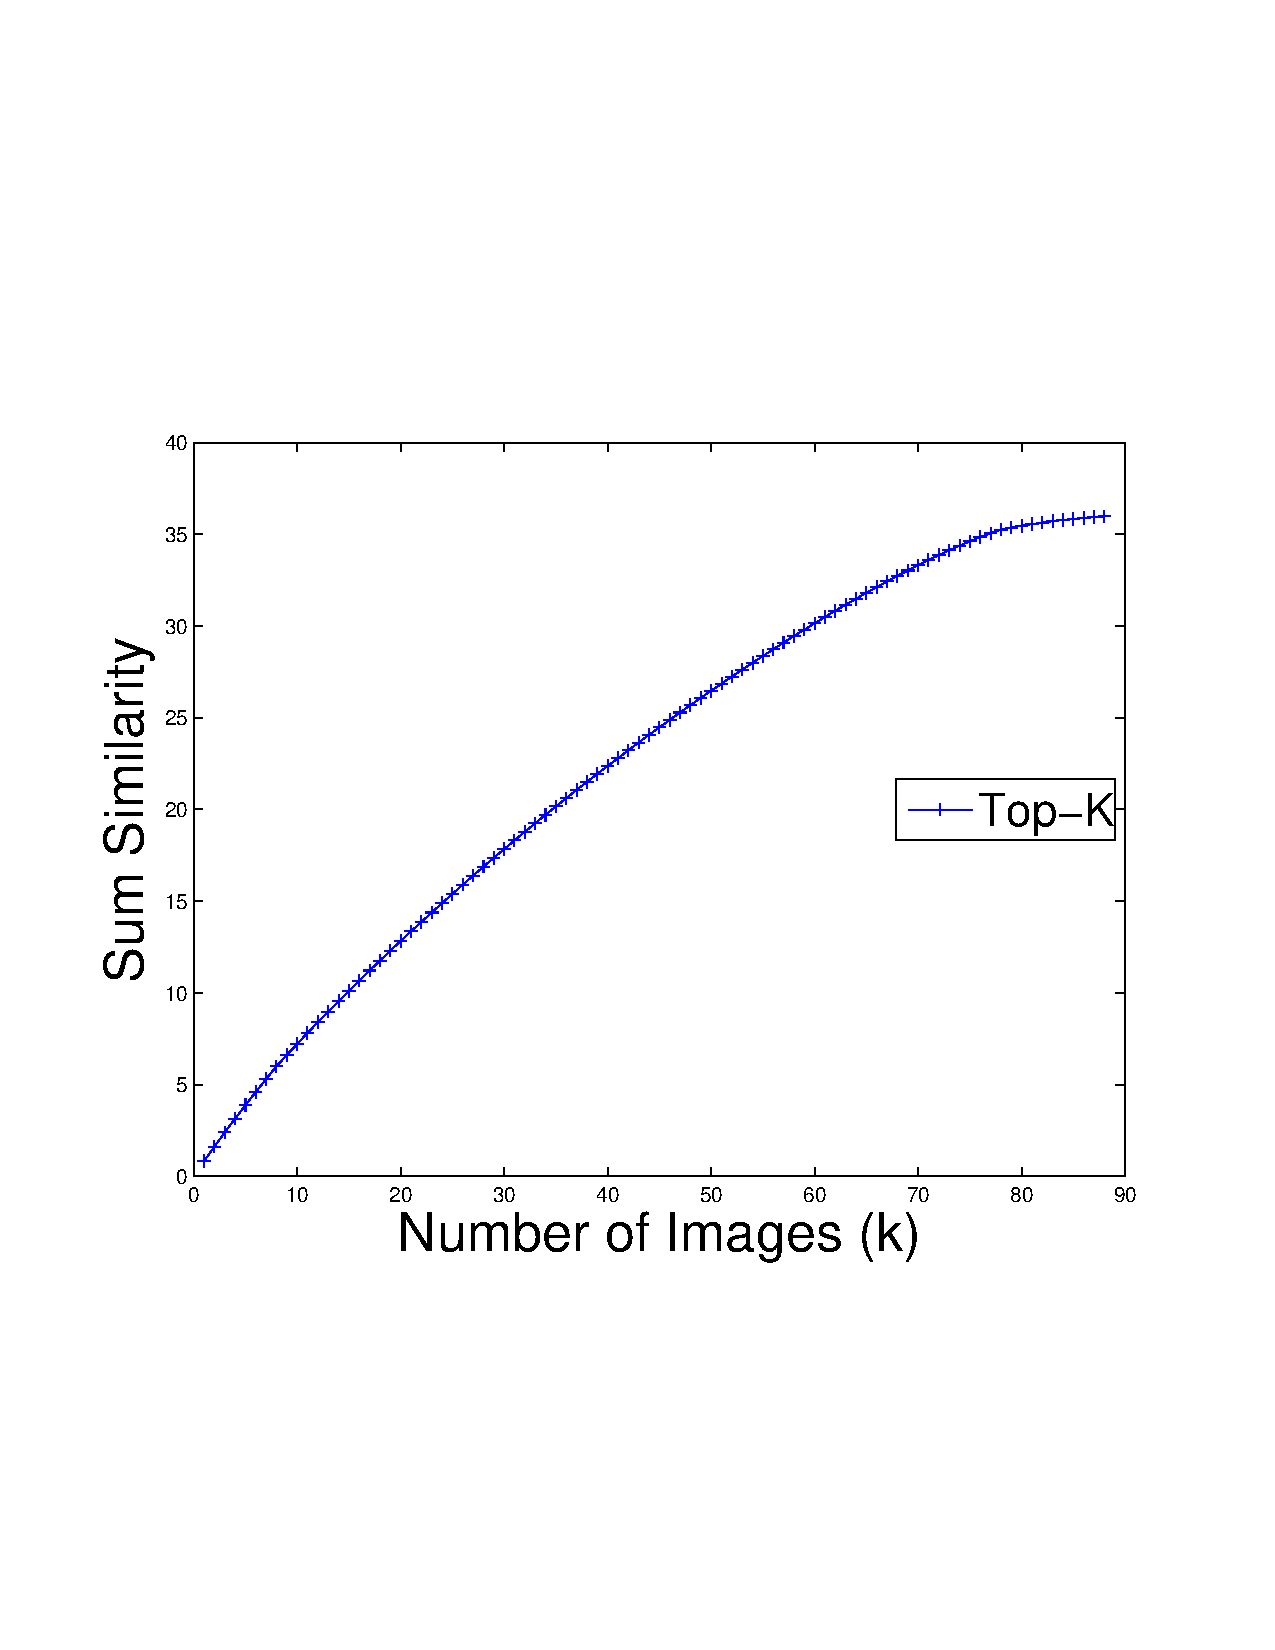
\includegraphics[clip=true, trim = 17mm 65mm 25mm 70mm, scale=0.23]{figures/topk/topk_sum_sim_color.pdf}
        \label{fig:topkSumSim}
        }
    \subfigure[Top-K: Avg. Match Target]{
        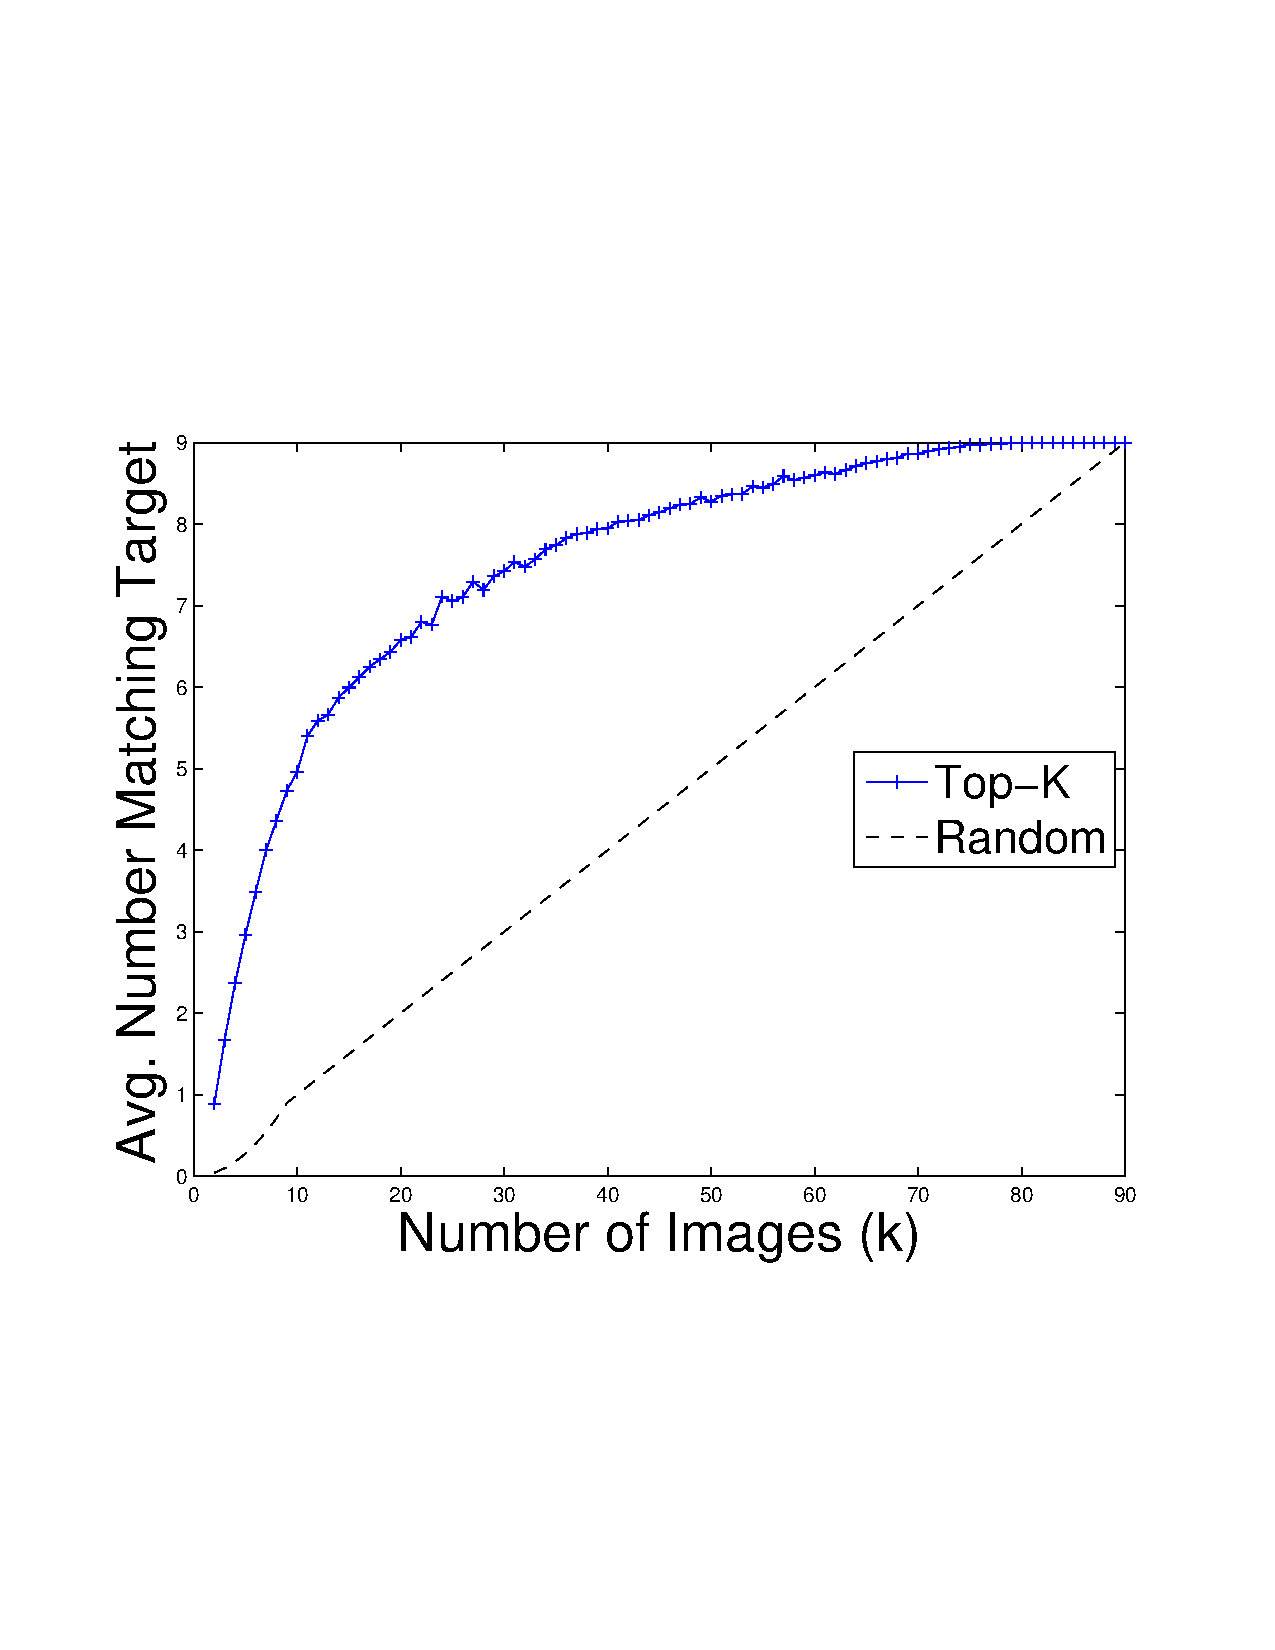
\includegraphics[clip=true, trim = 17mm 65mm 25mm 70mm, scale=0.23]{figures/topk/avg_num_matching_color.pdf}
        \label{fig:topkAvgNumSameSet}
        }
    \subfigure[Spanner: Sum Dissimilarity]{
        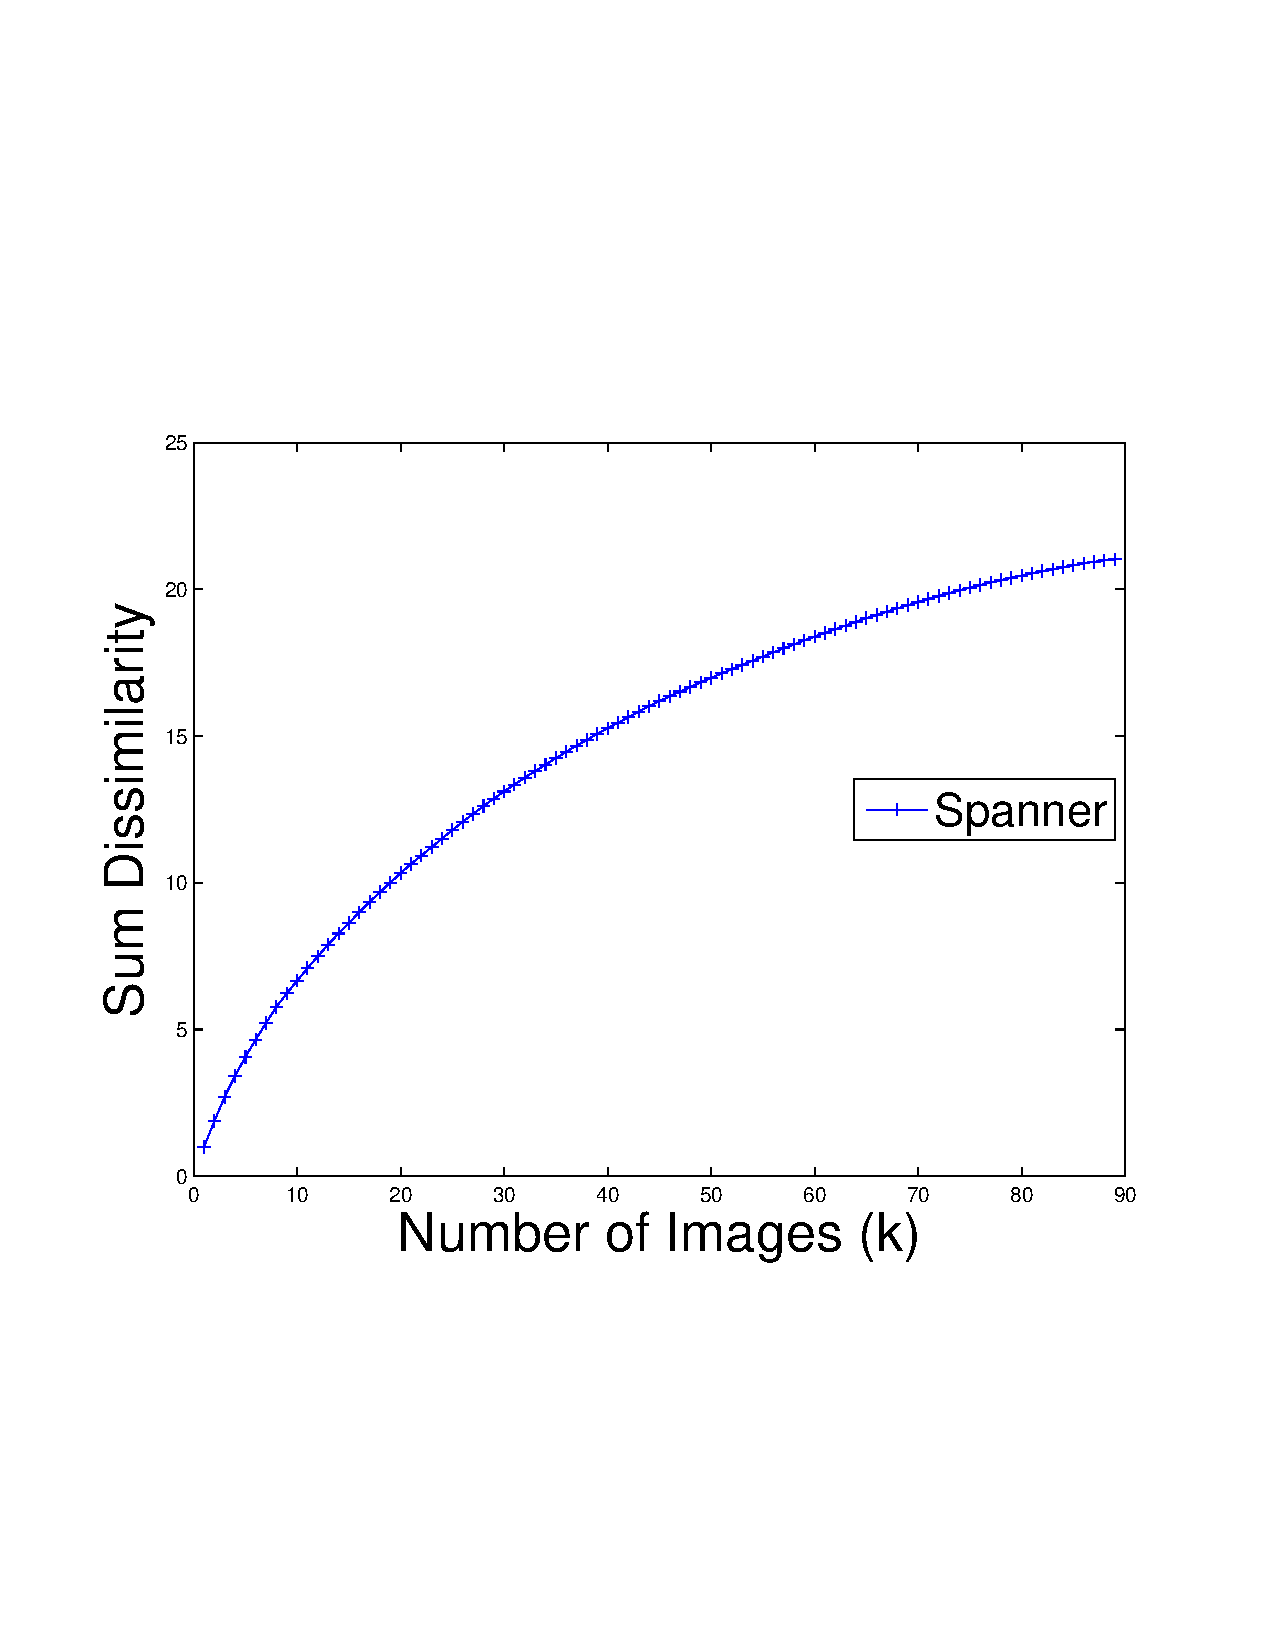
\includegraphics[clip=true, trim = 17mm 65mm 25mm 70mm, scale=0.23]{figures/spanner/spannerCumulativeDist_color.pdf}
        \label{fig:spanSumDissim}
        }
    \subfigure[Clustering: Cover All Sets]{
        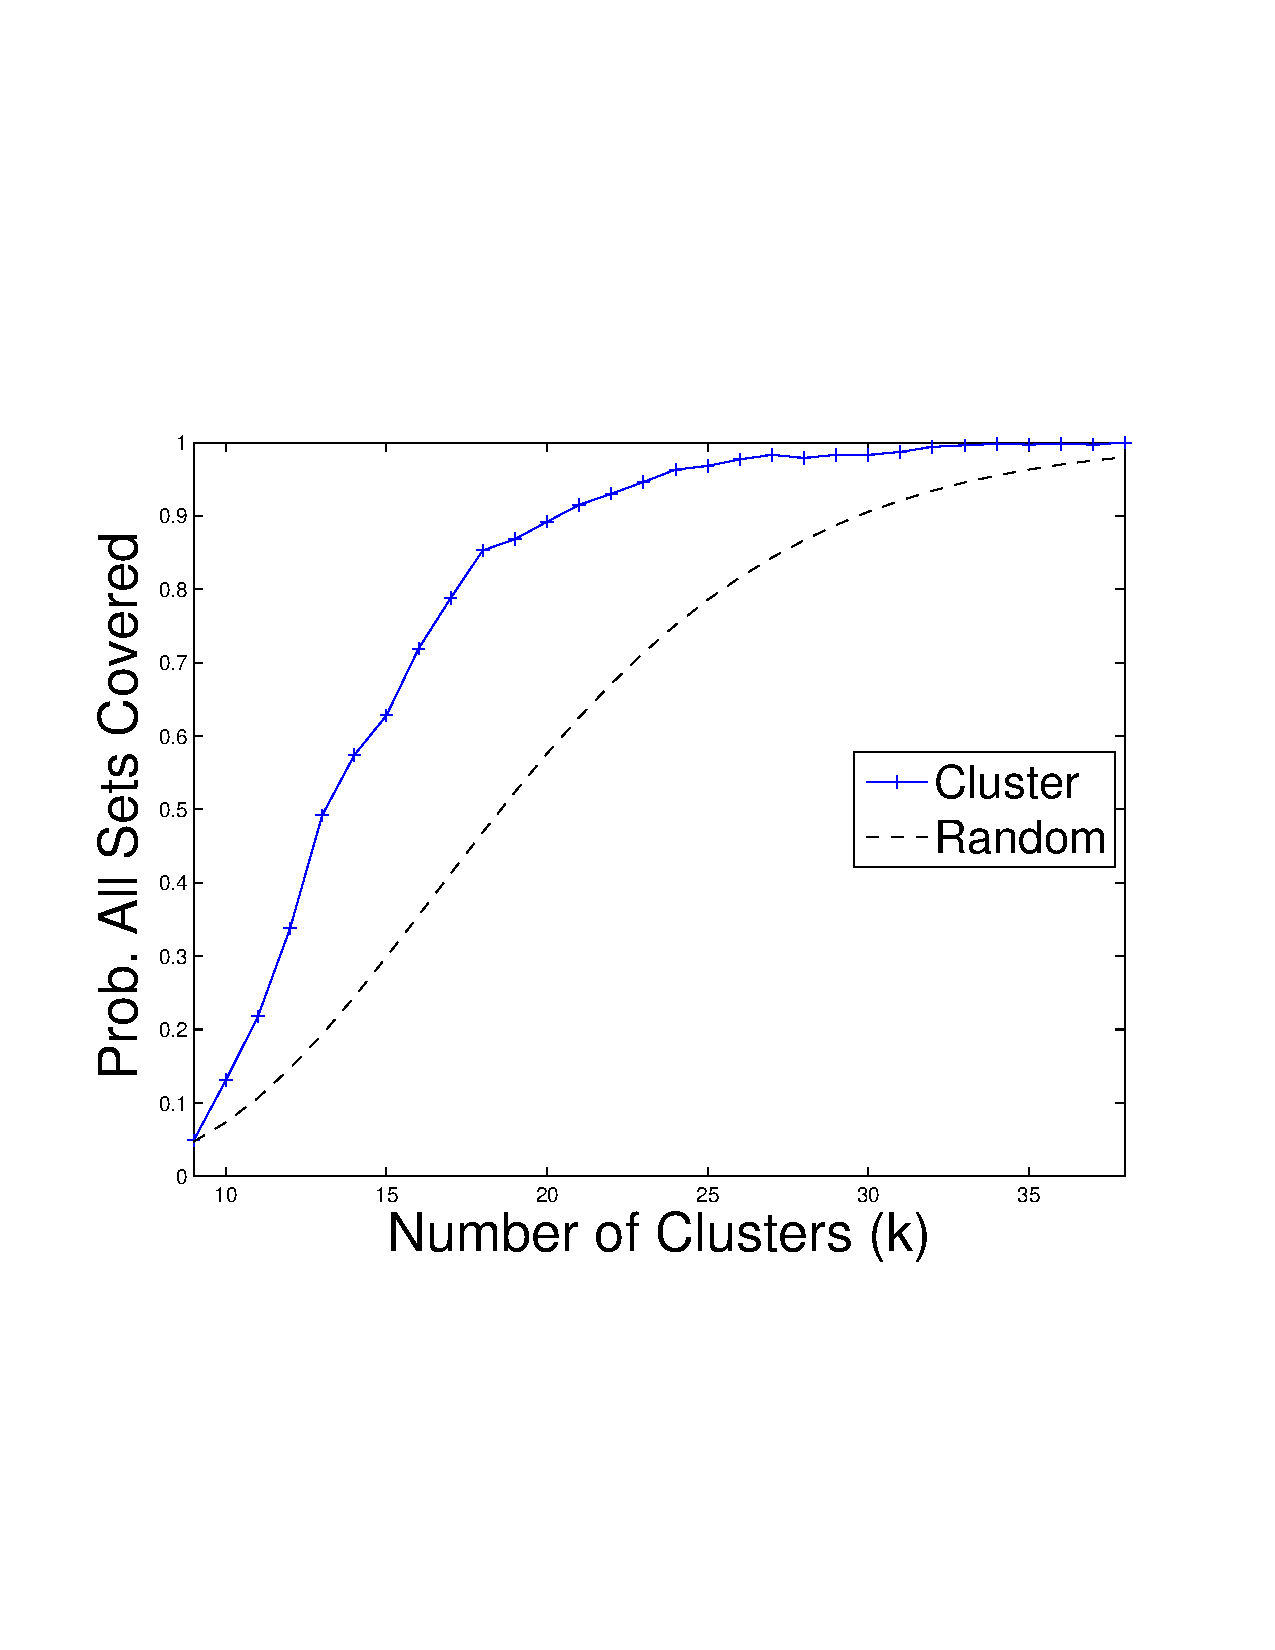
\includegraphics[clip=true, trim = 16mm 65mm 25mm 70mm, scale=0.23]{figures/cluster/perc_all_sets_covered_vary_k_color.pdf}
        \label{fig:clusterAvgNumSetsCov}
        }        
   \caption{Completeness metrics for the three image selection algorithms. Each exhibits a diminishing return as more images are added.}
   \label{fig:completeness_exp_results}
\end{figure*}

QoI is a multi-dimensional metric that can be defined for an application to give a more meaningful measure of the value of information.  It consists of attributes such as  timeliness, freshness, completeness, accuracy, precision, etc.  
For example, information that contributes to a decision-making process may only be useful if it arrives before the decision must be made, or it may have varying usefulness based on how similar or dissimilar it is to other data already collected.

The specific details of which attributes are considered and how they contribute to QoI is application-dependent.  Chosen QoI metrics are stored as a vector associated with a data item.  
Here, as in \cite{qoi_aware_tactical_mil_nets}, we specify a vector of minimum values for each QoI metric, and 
information is evaluated based on whether it satisfies all of the QoI requirements or not.  We use this approach to establish the edges of QoI satisfiability for the vector of metrics, which defines the boundaries of maximum achievable QoI regions in the metric space.

We choose to use two QoI attributes, one that is time-based and one that is information-content-based.  The first attribute is timeliness, $T$, of data.  For the second attribute, we present a notion of \emph{completeness}, $C$, which we show can be defined multiple ways, depending on the application and context.  Together, a QoI requirement of $\mathbf{q} = \{C,T\}$ specifies a quantity of data that must be delivered as well as a deadline by which it must arrive to be useful.  Since completeness is a rather new concept, we explain an example image selection algorithm and show how it can be evaluated with completeness.
%REFERENCES THAT USE COMPLETENESS: 1) mentions completeness of information in context of mobile sensor networks; argues that mobility can increase coverage/completeness \cite{qoi_data_collection_mobile_sens_nets};  

\subsection{Example Application: Similarity-based Image Retrieval}

As a motivating example, we choose a network in which nodes store photographs that are to be exchanged or collected at one or more data sinks.  This example covers surveillance missions of military tactical networks or camera sensor networks.  In this model, nodes can act as both clients and servers, issuing queries and serving images in response.  Therefore, as the network size increases, the amount of traffic is also likely to increase, but possibly disproportionately.  This fact exemplifies why the problem of characterizing the scalability limits for an instance is not straightforward.

To satisfy completeness of a query, we utilize measurements of the similarity or dissimilarity between pairs of images as explained in the rest of this section.  To get a similarity measurement, we use the same choice as was shown to be effective in \cite{mediascope}.  A technique called Color and Edge Directivity Descriptor (CEDD) \cite{2008cedd} provides a $54$-byte vector of qualities inherent to a photograph like lightness, contrast, and color.  The similarity between two images can then be given as a scalar by calculating the \emph{Tanimoto Similarity} \cite{tanimoto} between their CEDD vectors.  Dissimilarity is simply defined as $1$ minus the similarity.

\subsubsection{Selecting Similar Images}
One possible query for data is to retrieve images from the network that are similar to an identified target image.
The first type of query we introduce occurs when a user already has one image of a particular area or object of interest and would like to obtain similar images to get a more complete view of that specific scene or object.  
For example, if a user has a picture of an unknown suspicious person entering a building, but the person is not identifiable from that image, it would be useful to collect more images that are similar to that one with the possibility that another picture may have a better view of the person in question that can be used for identification or more context.  Called {\bf Top-K}, the query algorithm used for this application will choose the $k$ images with the most similarity with respect to the target image.  

We can evaluate the completeness of the result in one of two ways.  First, we can use the similarity of the images as a value representing each image's effectiveness in providing a more complete view of the target scene.  If we sum the similarity of all $k$ images returned by the algorithm, we get a representation of completeness, which we naturally call \emph{Sum Similarity}.  While this measure of completeness is abstract, it can be refined in an actual implementation through testing and evaluating.  This definition of completeness is useful, though, because it can be applied without any predetermined knowledge of the environment or pool of images.  

Often, though, we can partition the environment in which the network operates into a number, $n$, of distinct settings or areas.  In those cases, we can utilize a second method of quantifying completeness.  Assume that each image belongs to one of these $n$ sets, %$Q_i$, 
related to the setting it depicts.  Naturally, then, when executing a Top-K query, the goal is for the algorithm to return images from the same set as the target image.  Completeness can then be given by the fraction of images returned that are in the same set as the target image.

\subsubsection{Selecting Diverse Images}

In contrast, given the set of all photographs available in the network, we might want to return the set of $k$ images that exhibits the most diversity, ideally providing a user with a good sampling, or \emph{complete view}, of available images.  For instance, such a result would be quite useful in a surveillance mission.  We present two query algorithms that can be used to achieve this goal.

One query that provides diverse images is known as the {\bf Spanner} of the set of known photographs.  For the Spanner algorithm, we employ a greedy algorithm similar to that in \cite{mediascope}.  Here, the algorithm simply chooses images that provide the greatest minimum distance from all images already chosen.  This minimum distance can be added to a running sum to provide a completeness metric of \emph{Sum Dissimilarity}.  This value represents a measure of completeness because a higher level of dissimilarity provides a more complete view of the feature space.

%Here, the algorithm first chooses the two images with the greatest dissimilarity between them from all available images.  Then, each successive image is chosen to be the one with the greatest minimum distance between it and all images already chosen, until $k$ images are selected.  This minimum distance between the image being selected and the images in the collected set is the value added to the running cumulative completeness metric of \emph{Sum Dissimilarity}.  Since the Spanner algorithm's goal is to provide images at the edges of the available feature space, the Sum Dissimilarity represents a measure of its completeness because a higher level of dissimilarity is providing a more complete view of the feature space.

The other query that can achieve a complete view over all images is {\bf Clustering}.  In the Clustering algorithm, all images are separated into $k$ clusters based on their pairwise distances using any version of a k-means clustering algorithm, where $k$ is given by the user.  Then, the most central image from each cluster is returned.  
Here, assuming that the photographs of the same settings or objects of interest exhibit similar characteristics, 
Clustering also provides a complete view of the network's environment.

Both Spanner and Clustering algorithms can also be evaluated using a model assuming the environment is split into $n$ sets.  With this model, we can define completeness as either the number of sets represented by at least one of the $k$ images returned or the probability of all $n$ sets being represented by at least one image when $k$ are returned.  Here, though, we only show results for the second definition.

\subsection{Experimental Results}

To provide example values of these completeness metric definitions, experiments applying each query algorithm were run on a set of pictures taken at $n = 9$ different settings around the Penn State campus.  Each of these $9$ settings is of a pictorially different area, e.g. a particular building, a downtown street, or a lawn setting, and over $20$ images of each was taken.  Then, for individual trials, $10$ images from each set were randomly selected to create an image pool of $90$ pictures.  The three algorithms were run over these $90$ images, with the target image being randomly selected in the case of Top-K.  Results for each of the different completeness metrics were averaged over $1,000$ trials are shown in Figure \ref{fig:completeness_exp_results}. % Figures \ref{fig:topkSumSim} to \ref{fig:clusterAvgNumSetsCov}.

Figure \ref{fig:topkSumSim} shows the average sum similarity of images returned by the Top-K algorithm.  Figure \ref{fig:topkAvgNumSameSet} provides the second definition of completeness for the Top-K algorithm, the number of images matching the set that the target image was randomly chosen from.  Completeness results when dissimilarity is the objective are shown in Figures \ref{fig:spanSumDissim} and \ref{fig:clusterAvgNumSetsCov}.  Specifically, Figure \ref{fig:spanSumDissim} depicts the average Sum Dissimilarity returned by the Spanner algorithm, and Figure \ref{fig:clusterAvgNumSetsCov} represents the empirical probability of all $9$ sets being represented in the $k$ returned images.   For reference, we also include expected values for the metrics in Figures \ref{fig:topkAvgNumSameSet} and \ref{fig:clusterAvgNumSetsCov} if the images were selected from the entire image pool at random, i.e., without regard for image similarity or dissimilarity.  Details on these expected values given random selection are in Appendix \ref{sec:expl_exp_qoi}.

These figures exhibit the diminishing returns of completeness as more images are collected.  This effect visually shows how QoI differs from throughput.  As seen in these graphs, transmission of successive images does not result in a linear gain in completeness.  For example, in Figure \ref{fig:topkAvgNumSameSet}, it is evident that a value of only $k \approx 10$ is needed to collect $5$ images matching the target content, while collecting an additional $2$ from the same set usually requires collecting over twice that number of pictures.  
%For comparison, Figure \ref{fig:topkAvgNumSameSet} also shows the completeness achieved by random selection.
Similarly, Figure \ref{fig:clusterAvgNumSetsCov} shows that jumping from $k=10$ to $k=20$, the likelihood of capturing at least one image of every setting grows substantially from just over $10\%$ to approximately $90\%$.  To approach probabilities close to gaining that final $10\%$, however, requires a jump to $k\approx30$.  

The relationship between the number of images and completeness in each of these graphs also shows that obtaining a certain value of QoI or completeness requires a different number of images depending on the set available and their similarities.  We can denote the number of images required to achieve a level of completeness, $C$, as $k_{req} = Q(C)$.  This relationship will be useful later in determining capacity and scalability limits.

%\subsection{Other Applications}
%In our work, we also studied and experimented with two other algorithms in \cite{mediascope} that provide completeness by returning images that are dissimilar from each, providing a representative view of available data.  These completeness definitions resulted in very similar relationships as seen in Figure \ref{fig:completeness_exp_results} and are omitted for space.  We also note that the formulation in Section \ref{sec:qoi_scalability} is not restricted to just completeness, but can be used with any QoI metric that can be translated into a data requirement.
\subsection{Further Discussion of QoI}
We have defined and provided examples for a number of ways that completeness can be defined and used to obtain a concrete data requirement from a contextual QoI requirement.  Throughout the rest of the paper, we use sum similarity and the probability of covering all sets using clustering as completeness metrics, but we note that any of the definitions of completeness used here, or any other QoI requirement that can be translated into a data requirement, for that matter, can be used. % in the formulation in Section \ref{sec:qoi_scalability}.

%Also, note that QoI and its usage in understanding networks is not exclusive to these metrics and applications.  On the contrary, the model used in the capacity and scalability analysis of Section \ref{sec:qoi_scalability} is meant to be an in-depth example of this concept.  Modifications to account for different data size requirements should be quite straightforward, and extensions to other time-based metrics should be possible with careful extensions to the framework.

Also, while metadata associated with photographs may be useful in obtaining similar goals to those given in this section, relying on such information is problematic because metadata is not guaranteed to be available, and it is not as universally applicable as content-based retrieval.  For example, tags describing the image contents would require users to participate by entering this information, which is time-consuming and unreliable.  Location and time stamps may be automatically applied by the device allowing an application to filter images accordingly, but these tags often do not account for factors such as the direction of the camera or obstructed views.  Content-based processing, though, can be applied to any set of images.



